\documentclass[12pt,openright,oneside,a4paper,brazil]{abntex2}
\usepackage[utf8]{inputenc}
\counterwithout{section}{section}
\counterwithout{figure}{chapter}
\counterwithout{table}{chapter}
\setlength{\parindent}{1.3cm}
\usepackage{indentfirst}
\setlength{\parskip}{0.2cm}
\usepackage[bottom=2cm,top=3cm,left=3cm,right=2cm]{geometry}
\usepackage{graphicx}
\graphicspath{{figuras/}}
\usepackage{placeins}
\usepackage{cite}
\usepackage{url}
\usepackage{breakurl}

\makeatletter
\setlength{\@fptop}{0pt}
\makeatother

\begin{document}

\textual
\begin{center}
 {\large Captação de água e materiais estruturais}\\[0.2cm]
 \end{center}
 
Dentre as inspirações de tecnologia a serem aplicadas no projeto, as que se destacaram foram a Eolewater, Maxwater, Skywater e Warkawater. As três primeiras se baseiam no cooling compression, porém com custos diferentes. A Quarta tem custo  extremamente baixo se comparado com as outras Três tecnologias, por causa da simplicidade dos materiais que a constituem.Contudo, produz valores significantemente menores de água, além de não gerar energia para os processos de controle da qualidade da água. Por não gerar energia, também descartamos o Skywater.

As duas primeiras se baseiam em turbinas eólicas autossuficientes que retiram a umidade do ar, condensam, purificam e distribuem. Devido a geometria dos rotores do Max water que não é tão eficiente como os rotores tradicionais, de turbinas eólicas comuns, foi escolhido como base O sistema da Eolewater, que está descrito na figura 2.

\begin{figure}[!ht]
\centering
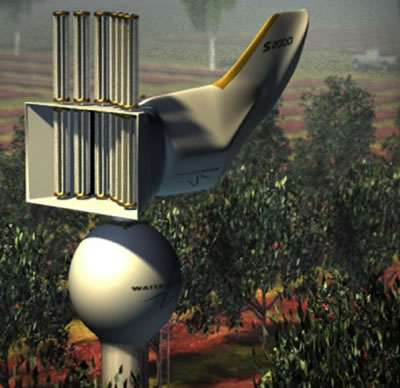
\includegraphics[scale=0.6]{max_water}
\caption[Caption title in LOF]{Max Water. Note como seus rotores são paralelos e verticais, tal configuração é ineficiente do ponto de vista aerodinâmico por gerar turbulência sobre os rotores vizinhos e gerar torques contrários com uma mesma direção de fluxo de ar.\footnotemark}

\label{Max_Water}
\end{figure}
\footnotetext{Disponível em: http://peswiki.com/index.php/Image:Max-water.jpg}

\begin{figure}[!htbp]
\centering
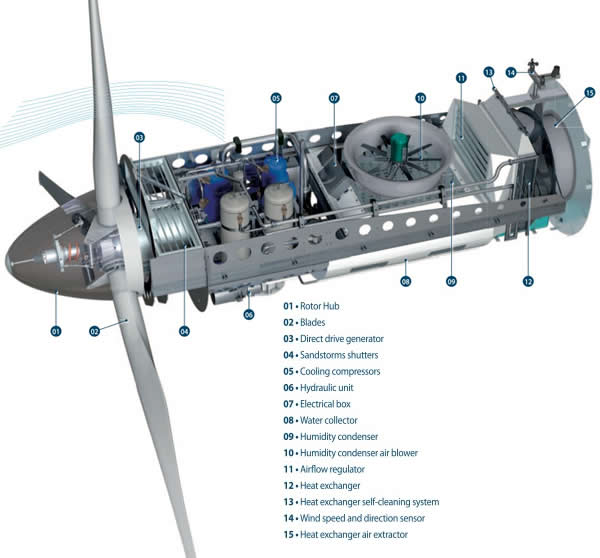
\includegraphics[scale=0.6]{Componentes}
\caption[Caption title in LOF]{Componentes de uma turbina Eolewater.\footnotemark}
\FloatBarrier
\label{Max_Water}
\end{figure}

\footnotetext{Fonte: RENEWABLE ENERGY DEVELOPMENT, 2012 }

As componentes de uma turbina eólica pouco mudam para essa acima,pois a Eolewater além de gerar energia para seu próprio funcionamento gera água, enquanto que a turbina eólica gera apenas energia.Na maioria das tecnologias de sucesso que pesquisamos, A Obtenção de água é feita pela condensação  a frio (cooling condensation), que é feita com o contato de ar com uma superfície fria. Para gerar essa superfície fria, são usados compressores e condensadores, refrigeradores básico, que pela segunda lei da termodinâmica, precisa de trabalho (Energia) para mover calor para do meio frio para o quente. Por isso, a necessidade da energia eólica não só para os sistemas de monitoramento e controle, como para a obtenção de água mais eficaz. 

No Momento, o levantamento de materiais será apenas estrutural e se baseará em uma turbina eólica.

\begin{figure}[!htbp]
\centering
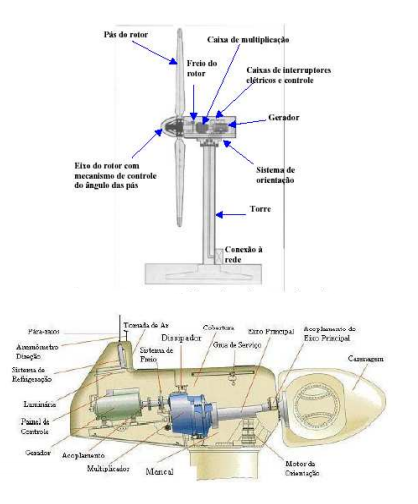
\includegraphics[scale=0.80]{turbina}
\caption[Caption title in LOF]{Seção de uma turbina eólica típica conectada à rede.\footnotemark}
\FloatBarrier
\label{Max_Water}
\end{figure}
\footnotetext{Fonte: USP, 2005 }

Dentro da turbina eólica temos os seguintes subconjuntos: torre, rotor, nacele, caixa de multiplicação (transmissão), gerador, mecanismos de controle, anemômetro, pás de rotor, biruta (sensor de direção). A torre é o elemento que sustenta o rotor e a nacele na altura adequada para o funcionamento da turbina eólica. Esse item é de elevada contribuição no custo inicial do sistema. O rotor é a componente onde as pás são conectadas e que realiza a transformação de energia cinética dos ventos em energia mecânica de rotação (ROSSI; OLIVEIRA; ALÉ, 2015).

	Nacele é um compartimento localizado no alto da torre que abrigam mecanismos do gerador (freios, caixa multiplicadora, embreagens, sistemas hidráulico, etc). Usaremos a Nacele para também abrigar os mecanismos de obtenção de água. 
	
	Caixa multiplicadora (transmissão) é o mecanismo que transmite a energia mecânica do eixo do rotar ao eixo do gerador. Gerador é o converterá energia mecânica do eixo em energia elétrica. Mecanismos de controle são os que supervisionam a velocidade média nominal que ocorre com maior frequência durante um determinado período. Anemômetro tem a função de medir a intensidade e a velocidade dos ventos. Pás do rotor captam o vento e converte sua potência ao centro do rotor. Biruta é um conjunto de sensores que captam a direção do vento \cite{wessberg2000real}.
	
	Uma das componentes que se tem muito estudo é a pá rotativa. Ela pode ser feita com os seguintes materiais: madeira, aço, alumínio, fibra de vidro com resina poliéster, fibra de vidro com fibra de carbono, madeira com epóxi, fibra de carbono. A escolha do material vai depender da escolha do perfil aerodinâmico, que será estudado posteriormente. (PORTAL ENERGIA, 2015).
\begin{figure}[!htbp]
\centering
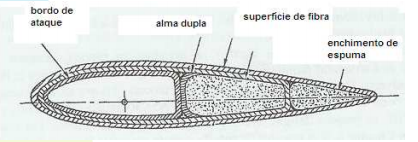
\includegraphics[scale=0.80]{pa}
\caption[Caption title in LOF]{Seção transversal de uma pá feita de fibra de vidro\footnotemark}
\FloatBarrier
\label{Max_Water}
\end{figure}
\footnotetext{Fonte: USP, 2005 }

Como pode ser visto as fibras são colocadas estruturalmente nas principais direções de propagação das tensões, quando em operação. A fibra de carbono e ou Kevlar são atualmente os compostos mais avançados que podem ser utilizados me áreas críticas (longarina da pá), mas tal material trem preços muito elevados (BARROS; VARELLA, 2015).  

Em relação ao suporte estrutural, ou torre, nas turbinas eólicas elas podem ser do tipo treliçadas, tubular e estaiada, no entanto, para a Eolewater as estruturas mais comuns são as duas últimas. As tores são constituídas de concreto e aço, tendo o peso em torno de 40 toneladas e 50 metros de comprimento (USP, 2005).

\begin{figure}[!htbp]
\centering
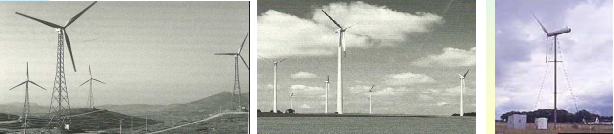
\includegraphics[scale=0.80]{torre}
\caption[Caption title in LOF]{Tipos de torre. Da esquerda para a direita: Treliçada, Tubular e Estaiada \footnotemark}
\FloatBarrier
\label{torre}
\end{figure}
\footnotetext{Fonte: USP, 2005 }

O modelo do dispositivo da Eolewater de gerar água por meio da energia eólica possui uma turbina WMS1000, de potência de30kW. O tempo de vida proposto para esse mecanismo é de 20 anos, dependendo das condições em que o motor é submetido ele pode gerar até 1200 litros de água por dia (mais informações na tabela abaixo). Como o dispositivo não necessita de quaisquer outros recursos para operar há um impacto mínimo sobre o meio em que é colocado (RENEWABLE ENERGY DEVELOPMENT, 2012).

\begin{figure}[!htbp]
\centering
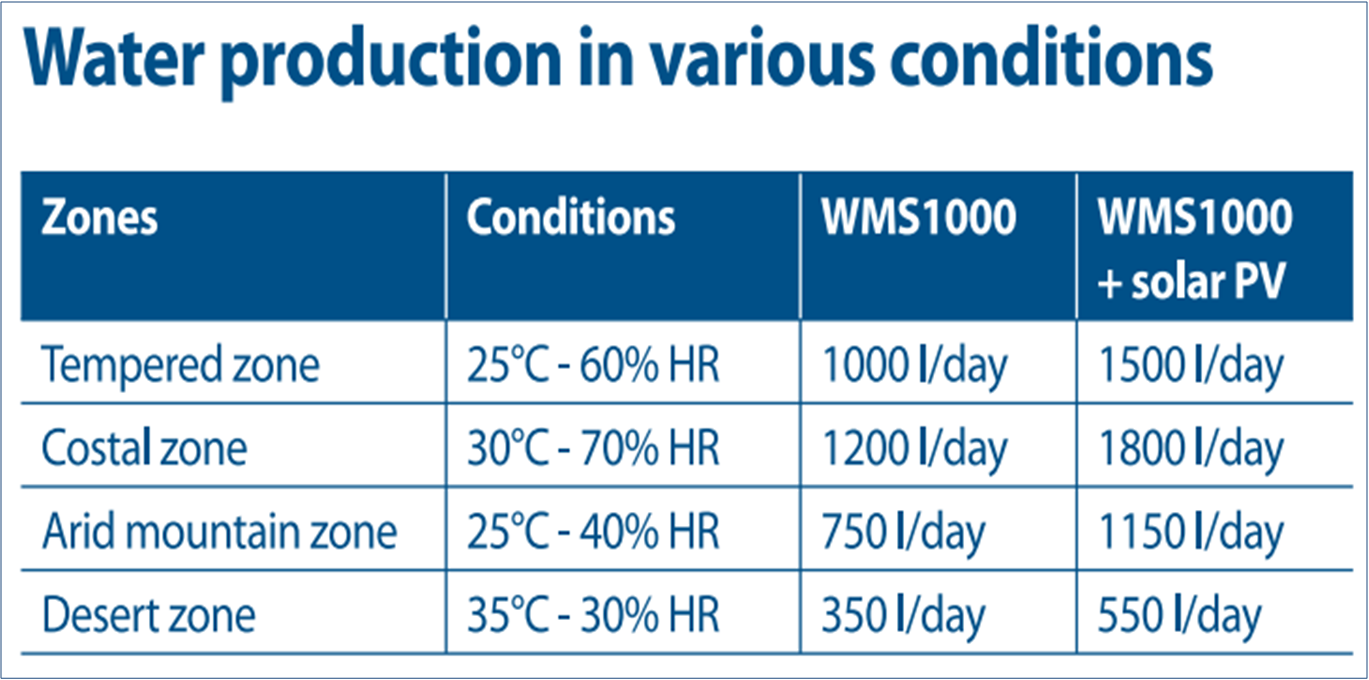
\includegraphics[scale=0.3]{condicoes}
\caption[Caption title in LOF]{Tabela de condições de umidade e temperatura para o rendimento de água \footnotemark}
\FloatBarrier
\label{condicoes}
\end{figure}
\footnotetext{Fonte: RENEWABLE ENERGY DEVELOPMENT, 2012}

Essa tecnologia possui um controle de pitch centrífuga para regular a velocidade do motor, tem um sistema de travagem rotor mecânica e elétrica, o qual evita danos nas lâminas giratórias (pás), ainda, contém um mastro de inclinação que integra a ação dos cilindros telescópicos com capacidade de empuxo de 115 toneladas. Deve-se destacar que os componentes que entram em contato com a água são feitos de uma liga de aço inoxidável especial que operará sem risco de corrosão (EOLE ÁGUA SAS, 2015).
	Uma tecnologia como essa segundo o site da Indústria Eólica uma turbina de vento abaixo de 100 kW vai custa por volta de US \$ 3.000 a US \$ 5.000  por quilowatt de capacidade. Portanto, levando em conta as especificações técnicas do Turbine WMS1000 abaixo a tecnologia é eficiente, mas cara (RENEWABLE ENERGY DEVELOPMENT, 2012).
	
\begin{figure}[!htbp]
\centering
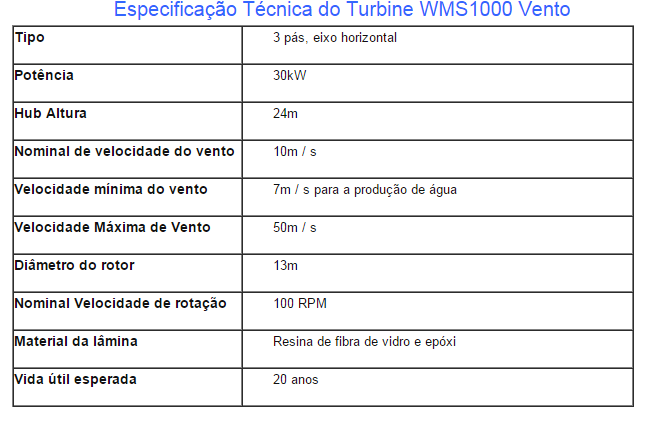
\includegraphics[scale=0.8]{especificacao}
\caption[Caption title in LOF]{Especificação Técnica do Turbine WMS1000 Vento \footnotemark}
\FloatBarrier
\label{Especificacoes}
\end{figure}
\footnotetext{Fonte: RENEWABLE ENERGY DEVELOPMENT, 2012}
 
A outra tecnologia, Warawater, por sua vez é uma tecnologia muito barata se comparada com a mencionada anterior. Essa custa cerca de US\$ 500 e pode ser construída em menos de uma semana com uma equipe de quatro pessoas e materiais existente localmente (DUARTE, 2015).
	Os materiais necessários para a sua construção de sua estrutura são: recipiente de coleta, bambu e um revestimento interno de plástico reciclado (rede). Sua torre possui em média 10 metros de altura, com 60 Kg e pode suprir até 100 litros de água por dia (TIMES, 2014).
\begin{figure}[!htbp]
\centering
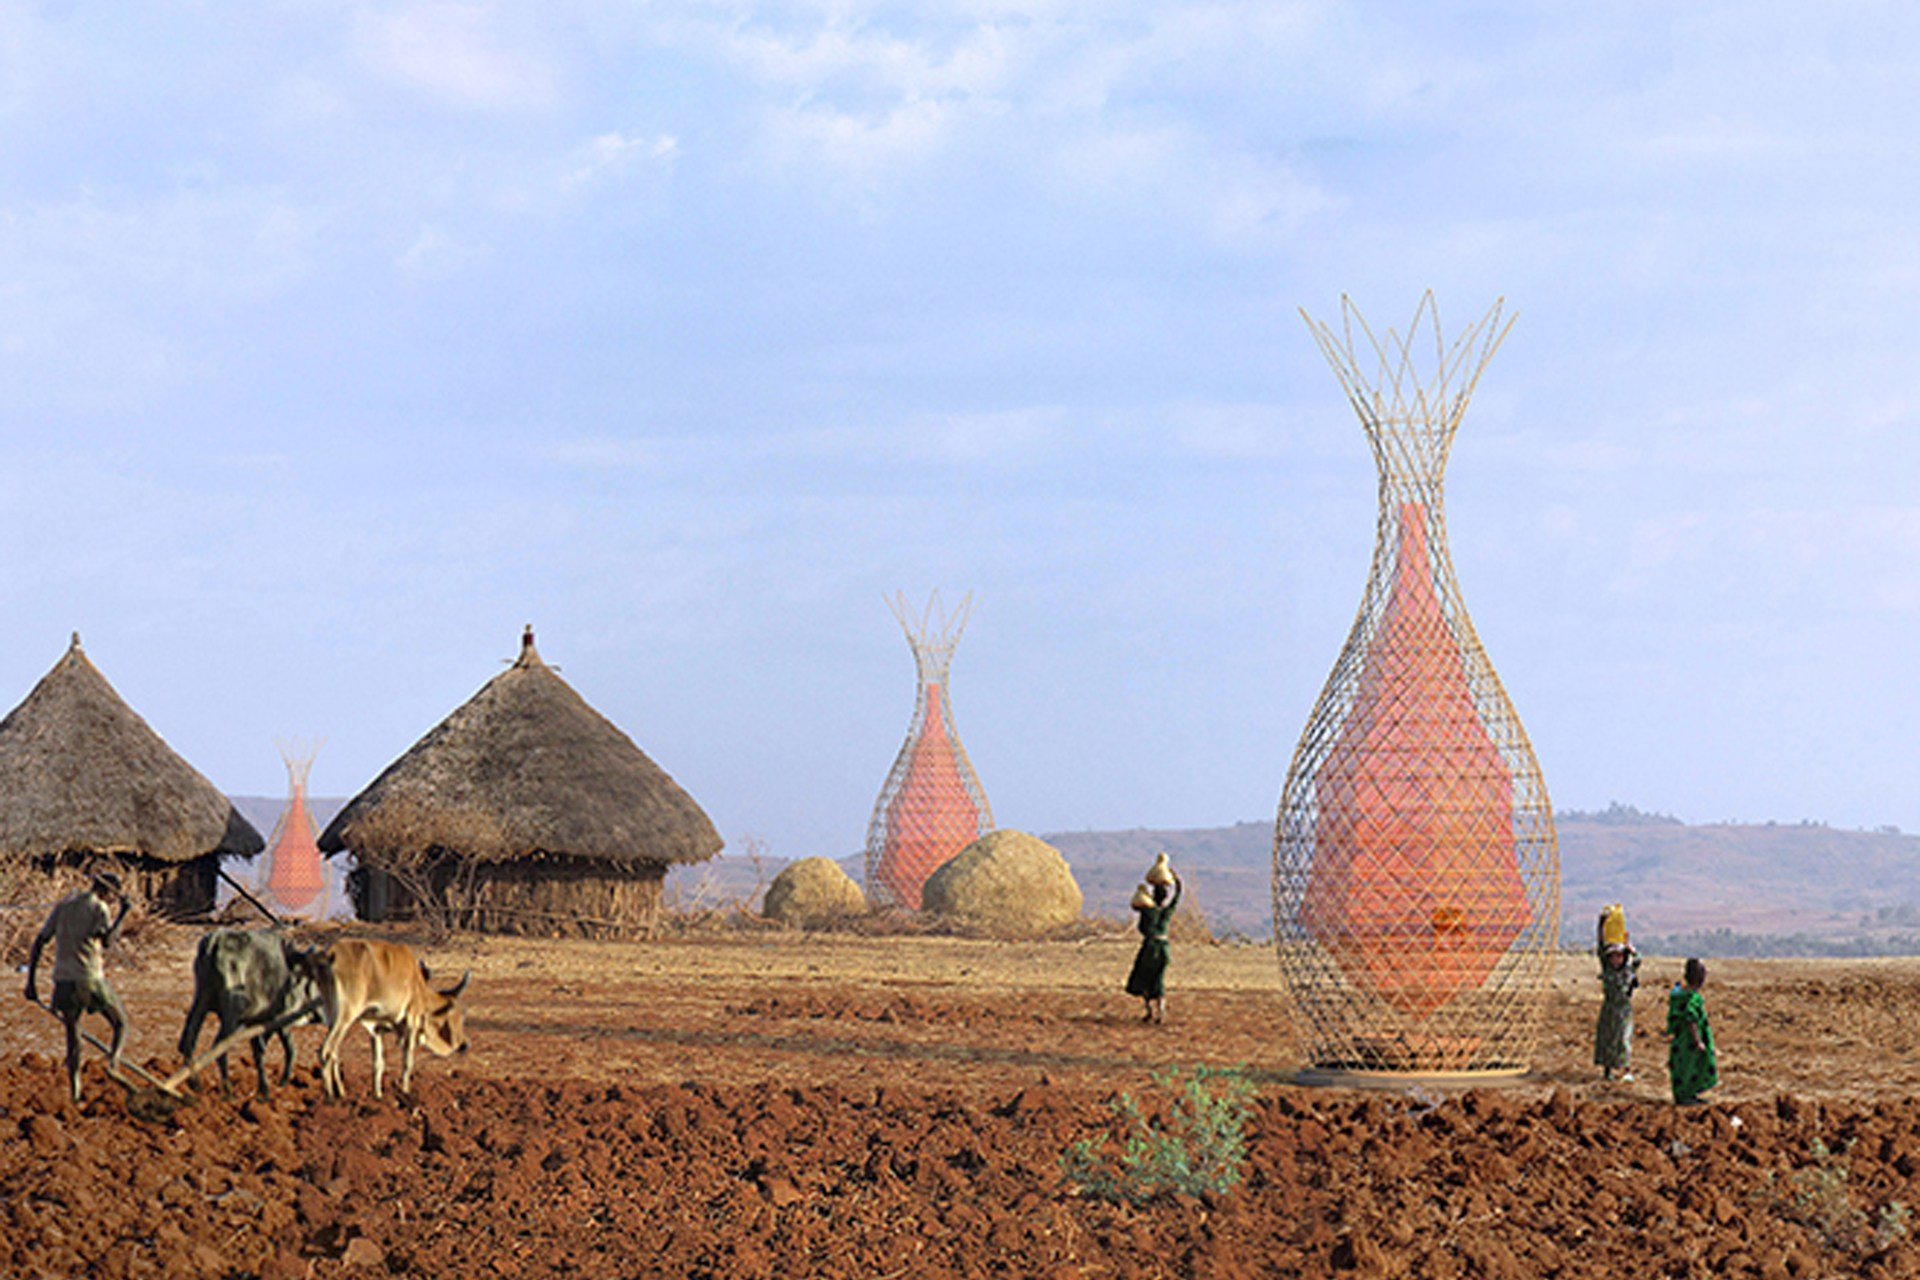
\includegraphics[scale=0.3]{warkawater}
\caption[Caption title in LOF]{Utilização da tecnologia warkawater por uma população carente  \footnotemark}
\FloatBarrier
\label{Especificacoes}
\end{figure}
\footnotetext{Fonte: DUARTE, 2015}

\bibliography{bibliografia}{}

\end{document}